\documentclass[conference]{IEEEtran}
\IEEEoverridecommandlockouts
% The preceding line is only needed to identify funding in the first footnote. If that is unneeded, please comment it out.
%Template version as of 6/27/2024

\usepackage{cite}
\usepackage{svg}
\usepackage{amsmath,amssymb,amsfonts}
\usepackage{algorithmic}
\usepackage{graphicx}
\usepackage{textcomp}
\usepackage{xcolor}
\def\BibTeX{{\rm B\kern-.05em{\sc i\kern-.025em b}\kern-.08em
    T\kern-.1667em\lower.7ex\hbox{E}\kern-.125emX}}
\begin{document}

\title{TODO}

\author{\IEEEauthorblockN{Daniël Jochems}
\IEEEauthorblockA{}
\and
\IEEEauthorblockN{David}
\IEEEauthorblockA{6787258}
\and
\IEEEauthorblockN{Niek Grimbergen}
\IEEEauthorblockA{1958413}
\and
\IEEEauthorblockN{Daan van Dam}
\IEEEauthorblockA{6434657}
}

\maketitle

\section{Introduction}
For this assignment we were given time series data and were tasked to train a deep learning model
to predict future values in this time series. In this report we will describe the methods we used 
to train our model, the results we obtained and the conclusions we drew from these results.

\section{Methods}
\subsection{Training data engineering}
First we prepare the timeseries data to accomodate lag features (past values of a variable at a
previous time step) using a lag-based sliding window approach. We do this by creating a new 
dataframe with the lagged values of the time series and dropping the rows with missing values.

Because the objective of this model is to predict future values of the time series, we need to
make sure that the model is trained on past values and validated on future values. Every fold the 
train fold grows by including the entire previous fold worth of data and adding the next fold's train fold.  
The validation fold remains the same size. The validation fold is structured in the following manner:
For a given time series of length $T$, we generate input-output pairs $(X_t,y_t)$ such that the 
input vector $X_t$ contains the previous $n$ observations $[x_{t-n}, x_{t-n+1}, \ldots, x_{t-1}]$ 
and the next value to be predicted is $\hat{y_k}$, which is the value at time $t$. $X_t$ is then 
updated by removing the first value and inserting $\hat{y_k}$ at the end of the vector giving us
$[x_{t-n+1}, \ldots, x_{t-1}, \hat{y_k}]$, and we predict the next value $\hat{y_{k+1}}$. This is 
repeated until the end of the validation fold is reached (see Figure \ref{fig:recursivecv}). This recursive structure of predicting 
values into the future by inlcuding already predicted values for subsequent predictions reflects 
the problem of predicting future values. 

\begin{figure}
    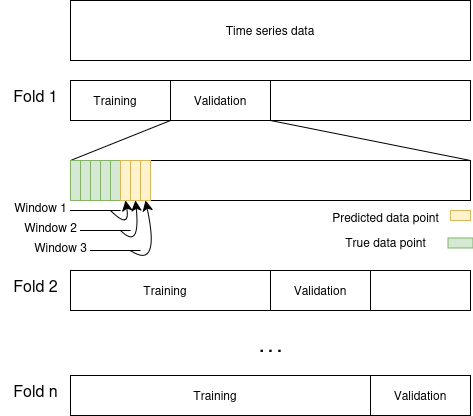
\includegraphics[scale = 0.47]{pictures/recursivecv.drawio.png}
    \caption{The recursive structure of the validation fold. The window of data points that are used 
    to predict the next value are shown. The first window being only true data points, subsequent windows
    inreasingly include predicted values until only predicted values are considered. The size of the 
    train fold increases with every fold, while the validation fold remains the same size.}
    \label{fig:recursivecv}
\end{figure}

%Every iteration we validate on the validation fold and save the metrics and an increasing weight. 
%The metrics over the folds are averaged taking into account these weights using the following
%formula:

%$$avg = \frac{\sum_{i=1}^{n}(\text{MSE}_{fold_n} * weight_n)}{\sum_{i=1}^n weight_n}$$

\subsection{LSTM}
We used a Long Short-Term Memory (LSTM) neural network to forecast our time series data, building on 
the architecture and tuning strategy described by Vien et al. \cite{kuen2021machine}. Since we are working 
with a univariate time series, the model was set up to predict future values based solely on past 
observations.

Before training, the library we used standardized the data using z-scores to ensure consistent scaling. We 
then performed a three-dimensional grid search to tune the model, exploring different combinations of the 
number of training epochs, the number of hidden units in the LSTM layer, and the number of lagged time 
steps used as input. This helped us find the setup that worked best for our dataset.

The LSTM architecture itself was straightforward: it included a sequence input layer, one LSTM layer with 
a tunable number of units, a fully connected layer, and an output layer. To evaluate the model, we used 
expanding window cross-validation (also known as forward-chaining), which ensured that the model was 
always tested on future data it hadn’t seen during training — an important detail for time series tasks.

We used mean absolute error (MAE) and mean squared error (MSE) to measure performance across folds. The 
final model was chosen based on the average error, weighted by the size of the training data in each fold.

\subsection{LTSM model parameter intialization}
For efficiency purposes we save time during our initial search for an appropriate number of epochs by 
fixing the number of hidden units to $15$ and lagged time steps to $25$. These values are the 'averages'
of the values we will iterate over during the later more extensive grid search. 
After we find the best epoch value we do another grid search over the number of hidden units and lagged
time steps. We use the same method as before, but now we fix the number of epochs to the best value
we found in the previous step. 

\subsection{LTSM model parameter intialization}
For efficiency purposes we save time during our initial search for an appropriate number of epochs by 
fixing the number of hidden units to $15$ and lagged time steps to $25$. These values are the 'averages'
of the values we we will iterate over during the later more extensive grid search. 

\section{Results}
TODO: This should be a sequence of statements each supported with some evidence and a conclusion.
Each statement is a subsection, the first paragraph of a statement summarizes the overall approach 
to solving the problem stated in the introduction, explain essential features of existing methods
we use and necessary background information. If we made a method ourselvers point it out clearly. 
Figures must be self contained (the legend and caption should have all the info for the figure).

\section{Discussion}
As described in our methods section we used a recursive approach to predict future values of the time series (see Figure \ref{fig:recursivecv}).
We did this for the entire validation folds length and use this "recursive loss" as a metric to evaluate the model. 
However it would have been interesting to compare this with a non-recursive approach, where we would predict the next 
value using only the true variables instead of the predicted values. That way you can't accumulate faults
made earlier.


\section*{AI statement}
GitHub Copilot was used to assist in writing this report. It was used to generate code snippets and
to help with the writing of the text. Moreover ChatGPT was used to format the single paper source as a 
'$\backslash$bibitem'.


\begin{thebibliography}{9}

    \bibitem{kuen2021machine}
    T. Kuen, L. R. F. Rose, W. K. Kong, and B. S. Vien,\\
    \textit{A machine learning approach for anaerobic reactor performance prediction using Long Short-Term Memory Recurrent Neural Network},\\
    Materials Research Proceedings, vol. 18, 2021.\\
    Publisher: Materials Research Forum LLC.
    
    \end{thebibliography}
    

\end{document}
